\chapter{A short guide to navigating phonon data}

PhonoPy is rich on features, check settings tags. Most things can be done without resorting to the python interface. There are, however a few caveats when we are interested in generating customized plots and working with eigenvectors.

\begin{enumerate}
    \item Check modulations with phonon website
    \item Use modulation feature of phonopy to generate desired modulations
    \item Python interface can be used to generate band structure plots
    \item Python interface can be used to generate $S(q,\omega)$
\end{enumerate}

\chapter{Phonon calculation formalism}
In most textbooks (e.g. Kittel \cite{Kittel2005}), phonon calculations are exemplified by simple models in one dimension consisting of only one or two inequivalent atoms. While these models are useful for providing basic results of lattice dynamical models, the extension to realistic models requires some level of abstraction. In particular, it is essential to cast the problem in terms of linear algebra. In this section, I will attempt to perform this abstraction starting from the diatomic chain. While software such as PHONON \cite{Parlinski1997} and Phonopy \cite{Togo2015} can be used without prior knowledge of the formalism, it is always useful to have some insights about our frequently used 'black boxes`.

\begin{figure}
    \centering
    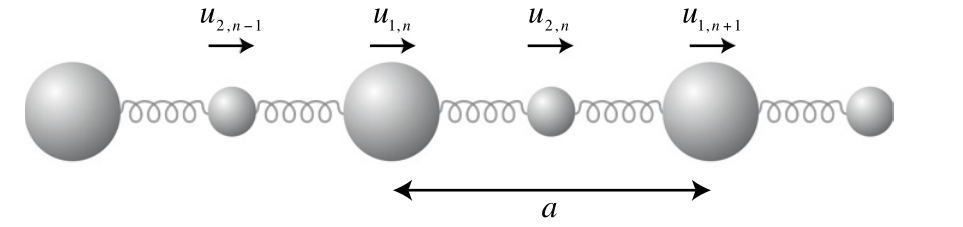
\includegraphics[width=0.9\textwidth]{fig/temp/diatomic.png}
    \caption{Diatomic chain}
    \label{fig:diatomic}
\end{figure}


The diamtomic chain is visualized in Figure \ref{fig:diatomic}. We consider an infinite chain of alternating ($1,2$) atoms with distinct masses ($m$,$M$) in a unit cell of length $a$. Displacements from equilibrium positions are denoted with $u_{i,n}$, where $n$ is the unit cell index. We start by making the assumption that the energy of this idealized lattice depends on the distance between pairs of atoms. If we consider the displacements $u$ to be small, the total energy of our chain can be expressed as a Taylor series

\[ E^\text{tot} = E_0 + \sum_i \frac{\partial E}{\partial u_{i}}  + \frac{1}{2} \sum_{i,j} u_{i} \frac{\partial ^2 E}{\partial u_{i} \partial u_{j}} u_{j} + \dots \, , \]

\noindent where the two indices $i$ and $j$ runs over all atomic species in the chain. To continue we first invoke the \emph{harmonic approximation} and ignore terms with power greater than 2 in the series. Second, we assume that the system is in equilibrium such that

\[ \frac{\partial E}{\partial u_{i}} = 0 \, , \]

\noindent for all values of $i$. Physically this corresponds to atoms being at rest in a parabolic (harmonic) potential. Since we are interested in  dynamics, it is convenient to use the \emph{harmonic energy} $E$ of the system

\[ E = E^\text{tot} - E_0 = \frac{1}{2} \sum_{i,j} u_{i} \frac{\partial ^2 E}{\partial u_{i} \partial u_{j}} u_{j} \]



